\section{Theoretischer Hintergrund}
Bei dem untersuchten Simulationsmodell handelt es sich um ein AC-PV-Batteriesystem, welches in \autoref{fig:plot1_230730333444} zu sehen ist. 
\begin{figure}[H]
    \centering
    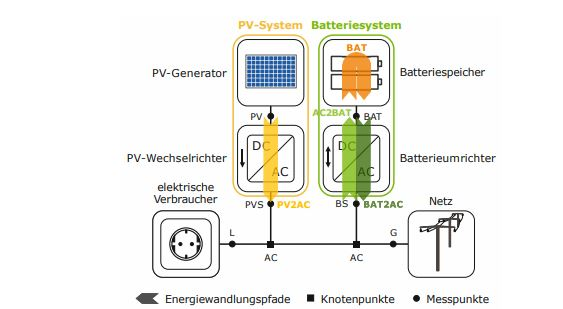
\includegraphics[width=\textwidth]{Abbildungen/12341234.jpg}
    \caption{Komponenten, Messpunkte und Energieumwandlungspfade bei AC-gekoppelten PV-Batteriesystemen.  [Versuchsanleitung]}
    \label{fig:plot1_230730333444}
\end{figure}
Für das PV-Batteriesystem sind vier wesentliche Komponenten erforderlich: der PV-Generator, der PV-Wechselrichter, der Batteriespeicher und der Batterie-Converter. Der PV-Generator wandelt Sonnenlicht in elektrische Energie um. Der PV-Wechselrichter dient dazu, den erzeugten Gleichstrom des PV-Generators in Wechselstrom umzuwandeln, der für den Haushaltsverbrauch geeignet ist.

Der Batteriespeicher ist für die Aufnahme und Speicherung der überschüssigen elektrischen Energie verantwortlich, die nicht sofort verbraucht wird. Der Batterie-Converter hat die besondere Eigenschaft, den Strom in beide Richtungen umzuwandeln, sodass er entweder in die Batterie geladen oder aus der Batterie entladen werden kann.

Durch diese Funktionalität ermöglicht der Batterie-Converter eine flexible Nutzung der erzeugten Energie. Der erzeugte Strom kann je nach Bedarf entweder direkt verbraucht, im Batteriespeicher gespeichert oder bei Bedarf ins Netz eingespeist werden, wenn die Batterie voll ist oder kein lokaler Verbrauch besteht. Dadurch kann das PV-Batteriesystem effizient Energie erzeugen, speichern und verwalten, um den Eigenverbrauch zu maximieren und den Bezug aus dem Netz zu reduzieren.


Des Weiteren sind die Fehlerquellen wichtig. Die Verluste haben dabei vor allem die folgenden 5 in \autoref{fig:plot1_230730333} Fehlerquellen.

\begin{figure}[H]
    \centering
    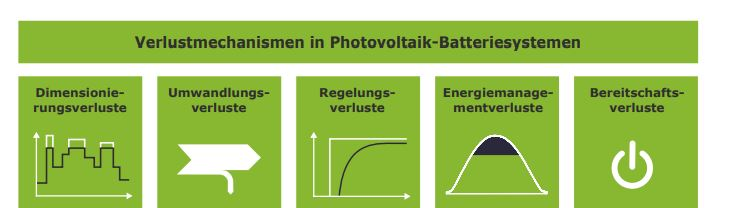
\includegraphics[width=\textwidth]{Abbildungen/aaa.jpg}
    \caption{Die fünf vorherrschenden Verlustmechanismen [Versuchsanleitung]}
    \label{fig:plot1_230730333}
\end{figure}
Die erste Verlustquelle, die Dimensionierungsverluste, ergeben sich beispielsweise durch eine zu geringe Auslegung bestimmter Komponenten wie Kabel oder Wechselrichter. Solche unterdimensionierten Komponenten können die Effizienz des Systems beeinträchtigen.

Die nächsten Verluste sind die Umwandlungsverluste. Diese treten auf, da der PV-Wechselrichter, der Batterieumrichter und die Batterie selbst den Strom stets umwandeln müssen. Diese Umwandlungsprozesse führen zu Energieverlusten.

Weiterhin entstehen Regelungsverluste durch Fehler in der Systemregelung, beispielsweise wenn die Batterie überschüssige Energie in das Netz einspeist oder Strom aus dem Netz bezieht. Solche Verluste können durch Messfehler und ungenaue Regelungsalgorithmen in der Realität auftreten.

Energiemanagementverluste resultieren aus der im Erneuerbare-Energien-Gesetz (EEG) festgelegten Regel, die die Einspeisung auf 70 \% der Nennleistung der PV-Anlage begrenzt. Dadurch können Verluste entstehen, wenn die Batterie bereits voll geladen ist und gleichzeitig viel Sonneneinstrahlung vorhanden ist. In einem solchen Fall muss die PV-Anlage gedrosselt werden, um die Einspeisung auf 70 \% zu begrenzen.

Und zuletzt treten Bereitschaftsverluste im Leerlauf- oder Bereitschaftsbetrieb auf und können durch den Einsatz von Stand-by- oder Schlafmodi minimiert werden. Dabei sollte darauf geachtet werden, dass die Leistungsaufnahme der einzelnen Systemkomponenten im Leerlauf möglichst gering gehalten wird, um unnötige Verluste zu vermeiden.  
